\documentclass{stdlocal}
\begin{document}
\section{Background} % (fold)
\label{sec:background}
  \subsection{Multiobjective Optimization} % (fold)
  \label{sub:multiobjective_optimization}
    The general goal of mathematical optimization is to quantify an optimal set of input parameters, which we call a configuration, that minimizes or maximizes a given cost function.
    For single-objective cost functions whose range is the space of real numbers, the natural total ordering of the real axis is intuitively used to decide which configuration leads to better results by comparing their outcome of the cost function.

    In multi-objective optimization the range of a cost function is multi-dimensional.
    Because there is no natural ordering of multi-dimensional real vector spaces, we have to clearly define what it means for a configuration to be more optimal than another one.
    \begin{definition*}[Domination]
      For $n\in\setNatural$, let $x,y\in \setReal^n$.
      Then we say $x$ dominates $y$ or $x\prec y$, if the following is true.
      \begin{enumerate}[label={(\arabic*)}]
        \item $\forall k\in\setNatural, k\leq m:\quad x_k\leq y_k$
        \item $\exists k\in\setNatural, k\leq m:\quad x_k < y_k$
      \end{enumerate}
    \end{definition*}
    This induces only a partial ordering for multi-dimensional spaces but seems to suffice for the typical optimization problems.
    Based on this definition, we can go even further and are able to define optimal values for multi-dimensional subsets.
    \begin{definition*}[Pareto Optimality]
      Let $n\in\setNatural$ and $X\subset\setReal^n$. A point $x\in X$ is said to be non-dominated or (Pareto) optimal, if there is no other point $y\in X$ which is dominating it.
      We denote $\mathrm{Pareto}(X)$ as the set of all (Pareto) optimal solutions in $X$.
    \end{definition*}
    With the concept of Pareto optimality, multi-objective optimization problems can be defined in the typical sense of single-objective optimization.
    \begin{definition*}[Multi-Objective Optimization Problem]
      Let $n\in\setNatural$ be the number of configuration variables, $m\in\setNatural$ with $m\geq 2$ be the number of objective values, and $X\subset\setReal^n$ the configuration space or the set of feasible solutions.
      Furthermore, let $\function{f}{X}{\setReal^m}$ be the cost function.
      Then we call the following the multi-objective optimization problem $\mathcal{P}$.
      \[
        \mathcal{P} \define \minimize_{x\in X} f(x)
      \]
      The solution $\mathcal{S}(\mathcal{P})$ to this problem is then given by the following subset of the graph of $f$ based on the configurations which map to the Pareto frontier.
      \[
        \mathcal{S}(\mathcal{P}) \define
        \set{(x,f(x))}{
        \begin{aligned}
          x &\in X, \\
          f(x) &\in \mathrm{Pareto}(\mathrm{im} f)
        \end{aligned}
        }
      \]
    \end{definition*}
    Typical multi-objective optimization problems which are also used as benchmarks for numerical solvers are given in table \ref{tab:pareto-two-objective-problems} and a visualization of their respective Pareto frontiers is given in figure \ref{fig:pareto-two-objective-problems}.

    \begin{figure*}[t]
      \center
      \begin{subfigure}[b]{0.24\textwidth}
        \center
        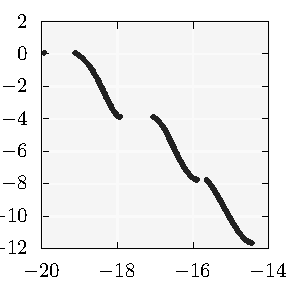
\includegraphics[width=\textwidth]{../../plots/kursawe.pdf}
        \caption{Kursawe}
      \end{subfigure}
      \begin{subfigure}[b]{0.24\textwidth}
        \center
        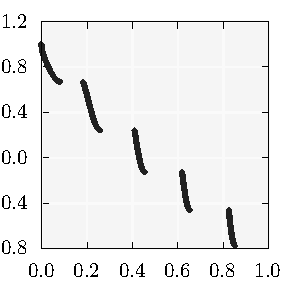
\includegraphics[width=\textwidth]{../../plots/zdt3.pdf}
        \caption{ZDT3}
      \end{subfigure}
      \begin{subfigure}[b]{0.24\textwidth}
        \center
        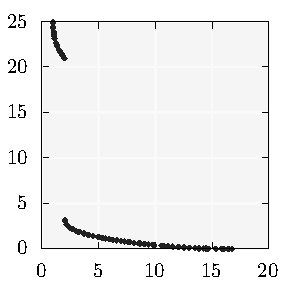
\includegraphics[width=\textwidth]{../../plots/poloni2.pdf}
        \caption{Poloni}
      \end{subfigure}
      \begin{subfigure}[b]{0.24\textwidth}
        \center
        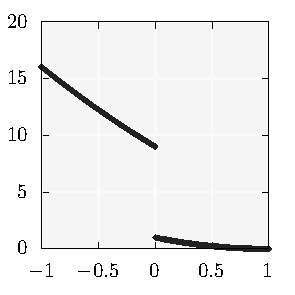
\includegraphics[width=\textwidth]{../../plots/schaffer2.pdf}
        \caption{Schaffer2}
      \end{subfigure}
      \caption[]{%
        These plots show the discontinuous Pareto frontiers of four standard two-objective test problems.
        All nondominated solutions were generated by using a custom C++ implementation of the NSGA-II algorithm according to \textcite{deb2002}.
      }
      \label{fig:pareto-two-objective-problems}
    \end{figure*}

    \begin{table*}
      \caption[]{%
        This table shows the mathematical formulation of the four standard two-objective test problems given in figure~\ref{fig:pareto-two-objective-problems}.
      }
      \label{tab:pareto-two-objective-problems}
      \hrule
      \smallskip
      \hrule
      \[
        \function{\text{Kursawe}}{[-5,5]^3}{\setReal^2}
        \separate
        \text{Kursawe}(x) \define
        \begin{pmatrix}
          \sum_{i=1}^2 -10 \exp\roundBrackets{-0.2 \sqrt{x_i^2 + x_{i+1}^2}} \\
          \\
          \sum_{i=1}^3 \absolute{x_i}^{0.8} + 5 \sin x_i^3
        \end{pmatrix}
      \]
      \hrule
      \[
        \function{\text{ZDT3}}{[0,1]^{30}}{\setReal^2}
        \separate
        \text{ZDT3}(x) \define
        \begin{pmatrix}
          x_1 \\
          \\
          g(x) \roundBrackets{1 - \sqrt{\frac{x_1}{g(x)}} - \frac{x_1}{g(x)} \sin 10π x_1}
        \end{pmatrix}
      \]
      \[
        g(x) \define 1 + \frac{9}{29}\sum_{i=2}^{30} x_i
      \]
      \hrule
      \[
        \function{\text{Poloni}}{[-π,π]^2}{\setReal^2}
        \separate
        \text{Poloni}(x) \define
        \begin{pmatrix}
          1 + [A - p(x)]^2 + [B - q(x)]^2 \\
          \\
          (x_1 + 3)^2 + (x_2 + 1)^2
        \end{pmatrix}
      \]
      \[
        A \define 0.5\sin 1 - 2 \cos 1 + \sin 2 - 1.5\cos 2
      \]
      \[
        B \define 1.5\sin 1 - \cos 1 + 2 \sin 2 - 0.5\cos 2
      \]
      \[
        p(x) \define 0.5 \sin x_1 - 2 \cos x_1 + \sin x_2 - 1.5 \cos x_2
      \]
      \[
        q(x) \define 1.5 \sin x_1 - \cos x_1 + 2 \sin x_2 - 0.5 \cos x_2
      \]
      \hrule
      \[
        \function{\text{Schaffer2}}{[-5,10]}{\setReal^2}
      \]
      \[
        \text{Schaffer2}(x) \define
        \begin{pmatrix}
          -x\mathds{1}_{(-\infty, 1]}(x) + (x-2)\mathds{1}_{(1,3]}(x) + (4-x)\mathds{1}_{(3,4]}(x) + (x-4)\mathds{1}_{(4,\infty)}(x) \\
          \\
          (x-5)^2
        \end{pmatrix}
      \]
      \hrule
      \smallskip
      \hrule
    \end{table*}

    \begin{figure*}[t]
      \center
      \begin{subfigure}[b]{0.24\textwidth}
        \center
        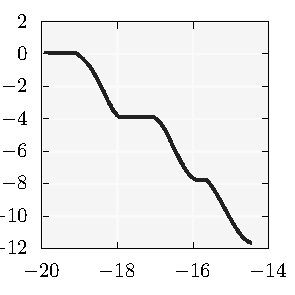
\includegraphics[width=\textwidth]{../../plots/kursawe_wrong.pdf}
        \caption{Kursawe}
      \end{subfigure}
      \begin{subfigure}[b]{0.24\textwidth}
        \center
        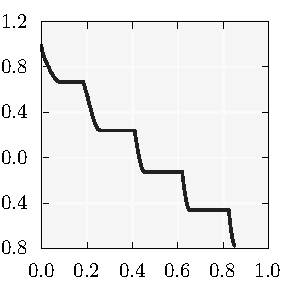
\includegraphics[width=\textwidth]{../../plots/zdt3_wrong.pdf}
        \caption{ZDT3}
      \end{subfigure}
      \begin{subfigure}[b]{0.24\textwidth}
        \center
        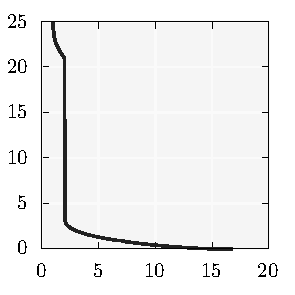
\includegraphics[width=\textwidth]{../../plots/poloni2_wrong.pdf}
        \caption{Poloni}
      \end{subfigure}
      \begin{subfigure}[b]{0.24\textwidth}
        \center
        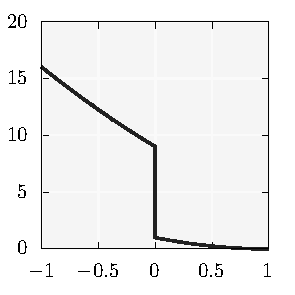
\includegraphics[width=\textwidth]{../../plots/schaffer2_wrong.pdf}
        \caption{Schaffer2}
      \end{subfigure}
      \caption[]{%
        These plots show the naive linear interpolation schemes for the two-objective test problems given by figure \ref{fig:pareto-two-objective-problems}.
        Discontinuities of the Pareto frontier are completely ignored.
        A configurator based solely on linear interpolation would provide impossible solutions.
      }
      \label{fig:pareto-two-objective-problems-wrong}
    \end{figure*}

    \begin{figure*}[t]
      \center
      \begin{subfigure}[b]{0.24\textwidth}
        \center
        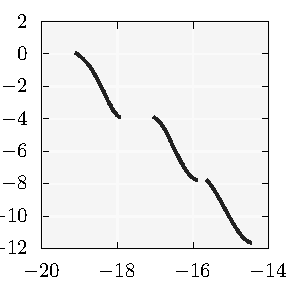
\includegraphics[width=\textwidth]{../../plots/kursawe_1000_tessellation.pdf}
        \caption{Kursawe}
      \end{subfigure}
      \begin{subfigure}[b]{0.24\textwidth}
        \center
        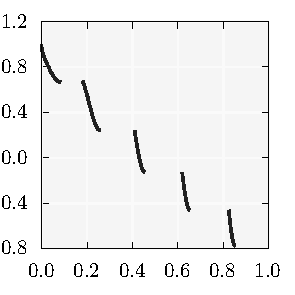
\includegraphics[width=\textwidth]{../../plots/zdt3_tessellation.pdf}
        \caption{ZDT3}
      \end{subfigure}
      \begin{subfigure}[b]{0.24\textwidth}
        \center
        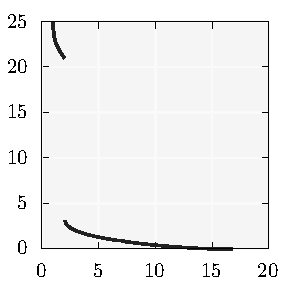
\includegraphics[width=\textwidth]{../../plots/poloni2_tessellation.pdf}
        \caption{Poloni}
      \end{subfigure}
      \begin{subfigure}[b]{0.24\textwidth}
        \center
        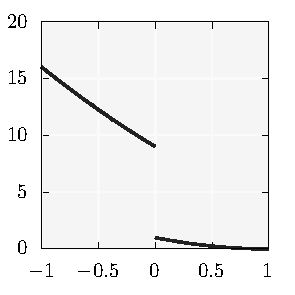
\includegraphics[width=\textwidth]{../../plots/schaffer2_tessellation.pdf}
        \caption{Schaffer2}
      \end{subfigure}
      \caption[]{%
        These plots show the linear interpolation schemes for the two-objective test problems given by figure \ref{fig:pareto-two-objective-problems} after applying the statistical heuristic to remove connections between neighboring points that may possibly exhibit discontinuities.
        For all examples, exactly those connections were removed that actually interpolated over a discontinuity.
      }
      \label{fig:pareto-two-objective-problems-tessellation}
    \end{figure*}

    \begin{figure*}[t]
      \center
      \begin{subfigure}[b]{0.24\textwidth}
        \center
        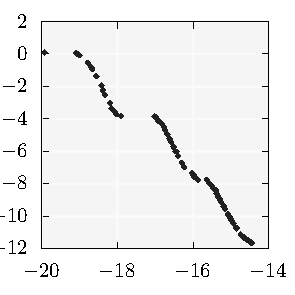
\includegraphics[width=\textwidth]{../../plots/kursawe_100.pdf}
        \caption{100}
      \end{subfigure}
      \begin{subfigure}[b]{0.24\textwidth}
        \center
        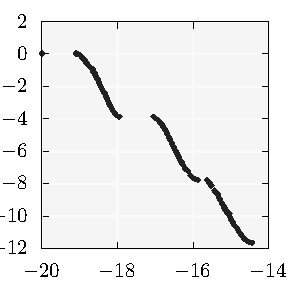
\includegraphics[width=\textwidth]{../../plots/kursawe_200.pdf}
        \caption{200}
      \end{subfigure}
      \begin{subfigure}[b]{0.24\textwidth}
        \center
        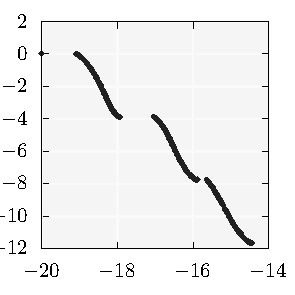
\includegraphics[width=\textwidth]{../../plots/kursawe_400.pdf}
        \caption{400}
      \end{subfigure}
      \begin{subfigure}[b]{0.24\textwidth}
        \center
        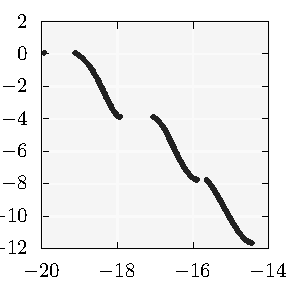
\includegraphics[width=\textwidth]{../../plots/kursawe_1000.pdf}
        \caption{1000}
      \end{subfigure}
      \caption[]{%
        These plots show the estimated Pareto frontier of the Kursawe problem given in table~\ref{tab:pareto-two-objective-problems} and shown in figure~\ref{fig:pareto-two-objective-problems} for different population sizes used in the underlying algorithm.
        All nondominated solutions have been computed by using a custom implementation of the NSGA-II algorithm according to \textcite{deb2002}.
      }
      \label{fig:kursawe-pareto-front-samples}
    \end{figure*}

    \begin{figure*}[t]
      \center
      \begin{subfigure}[b]{0.24\textwidth}
        \center
        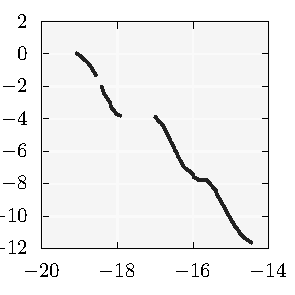
\includegraphics[width=\textwidth]{../../plots/kursawe_100_tessellation.pdf}
        \caption{100}
      \end{subfigure}
      \begin{subfigure}[b]{0.24\textwidth}
        \center
        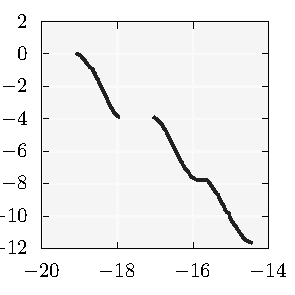
\includegraphics[width=\textwidth]{../../plots/kursawe_200_tessellation.pdf}
        \caption{200}
      \end{subfigure}
      \begin{subfigure}[b]{0.24\textwidth}
        \center
        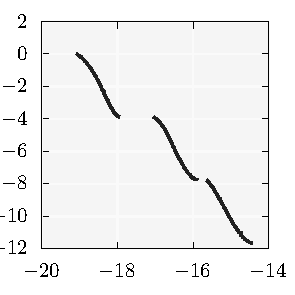
\includegraphics[width=\textwidth]{../../plots/kursawe_400_tessellation.pdf}
        \caption{400}
      \end{subfigure}
      \begin{subfigure}[b]{0.24\textwidth}
        \center
        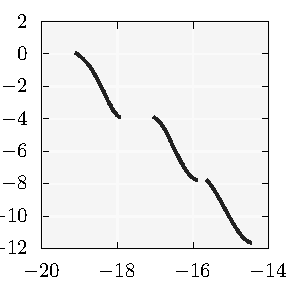
\includegraphics[width=\textwidth]{../../plots/kursawe_1000_tessellation.pdf}
        \caption{1000}
      \end{subfigure}
      \caption[]{%
        These plots show the linear interpolation schemes for Pareto frontier of the Kursawe problem shown in figure \ref{fig:kursawe-pareto-front-samples} after applying the statistical heuristic to remove connections between neighboring points that may possibly exhibit discontinuities.
        Due to the coarse grid of nondominated points for 100 and 200 samples in the population size, the given heuristic was not able to find all discontinuities and even removed a valid connection for 100 samples.
      }
      \label{fig:kursawe-pareto-front-tessellation}
    \end{figure*}

    \begin{figure*}[t]
      \center
      \begin{subfigure}[b]{0.24\textwidth}
        \center
        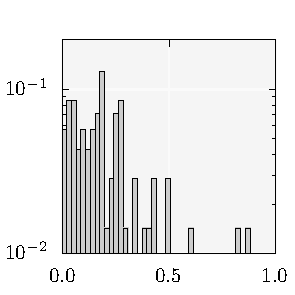
\includegraphics[width=\textwidth]{../../plots/kursawe_histogram_100.pdf}
        \caption{100}
      \end{subfigure}
      \begin{subfigure}[b]{0.24\textwidth}
        \center
        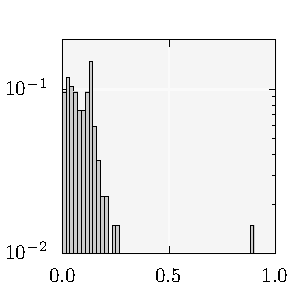
\includegraphics[width=\textwidth]{../../plots/kursawe_histogram_200.pdf}
        \caption{200}
      \end{subfigure}
      \begin{subfigure}[b]{0.24\textwidth}
        \center
        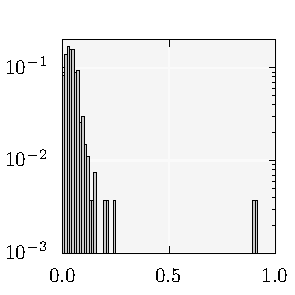
\includegraphics[width=\textwidth]{../../plots/kursawe_histogram_400.pdf}
        \caption{400}
      \end{subfigure}
      \begin{subfigure}[b]{0.24\textwidth}
        \center
        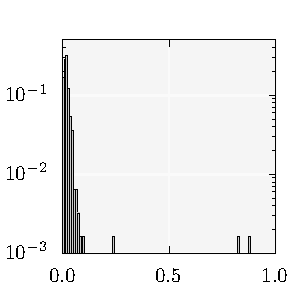
\includegraphics[width=\textwidth]{../../plots/kursawe_histogram_1000.pdf}
        \caption{1000}
      \end{subfigure}
      \caption[]{%
        These plots show the relative frequency histograms of distance distribution of neighboring points in the Pareto frontier of the Kursawe problem for different population sizes according to figure~\ref{fig:kursawe-pareto-front-samples}.
      }
      \label{fig:kursawe-histogram-samples}
    \end{figure*}
  % subsection multiobjective_optimization (end)
  \subsection{Delaunay Triangulation} % (fold)
  \label{sub:delaunay_triangulation}
    \begin{figure}
      \center
      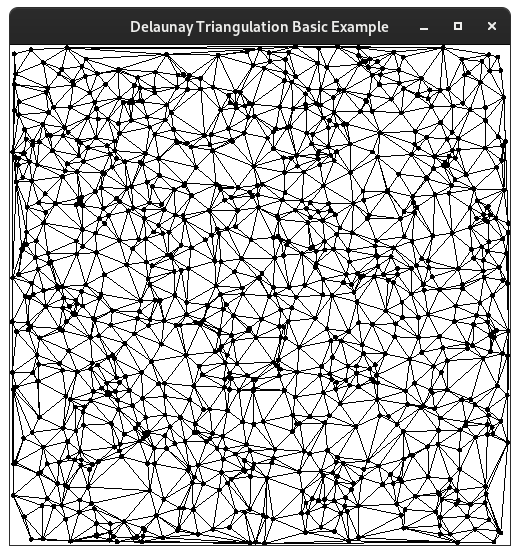
\includegraphics[width=0.35\textwidth]{../../images/delaunay_2d.png}
    \end{figure}
    \begin{figure*}
      \center
      \begin{subfigure}[b]{0.49\textwidth}
        \center
        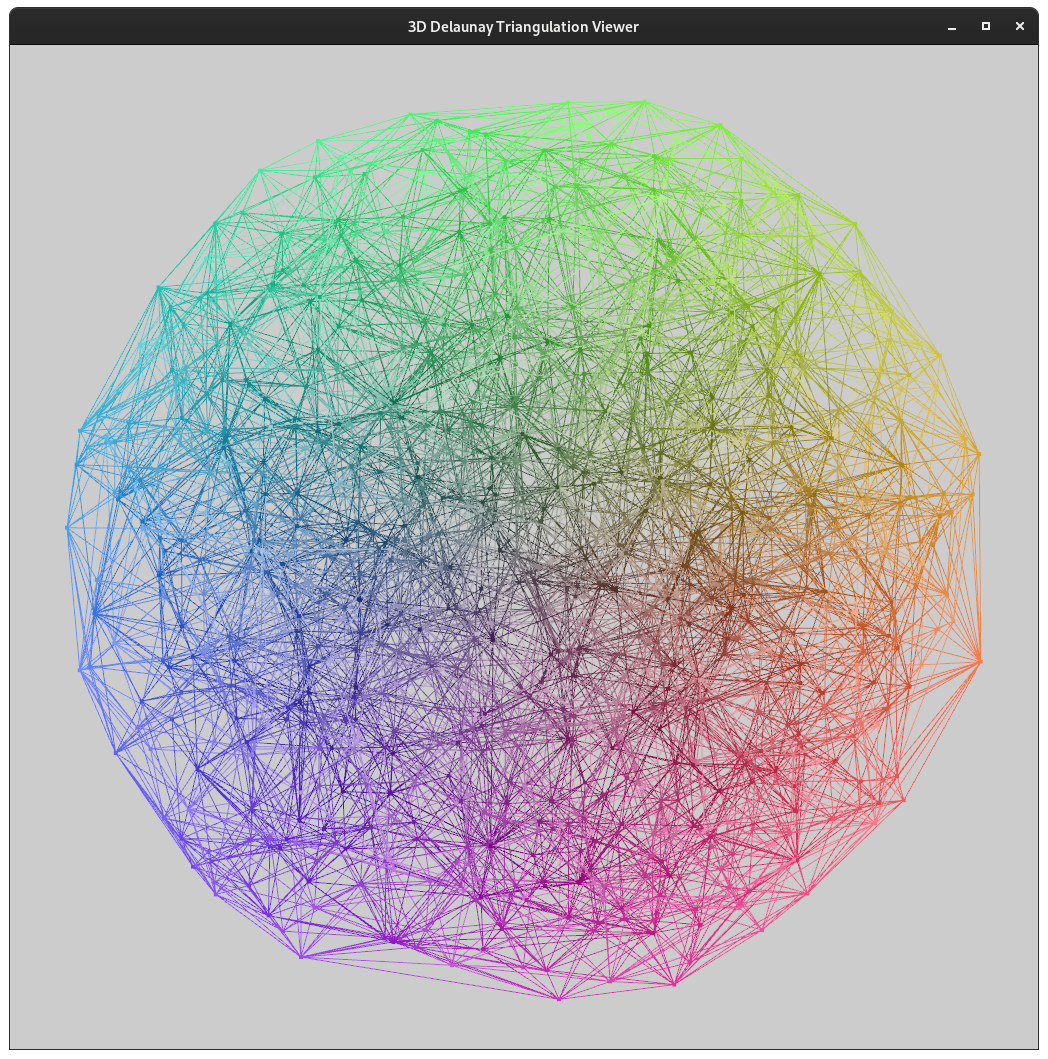
\includegraphics[width=0.8\textwidth]{../../images/delaunay_3d.png}
      \end{subfigure}
      \begin{subfigure}[b]{0.49\textwidth}
        \center
        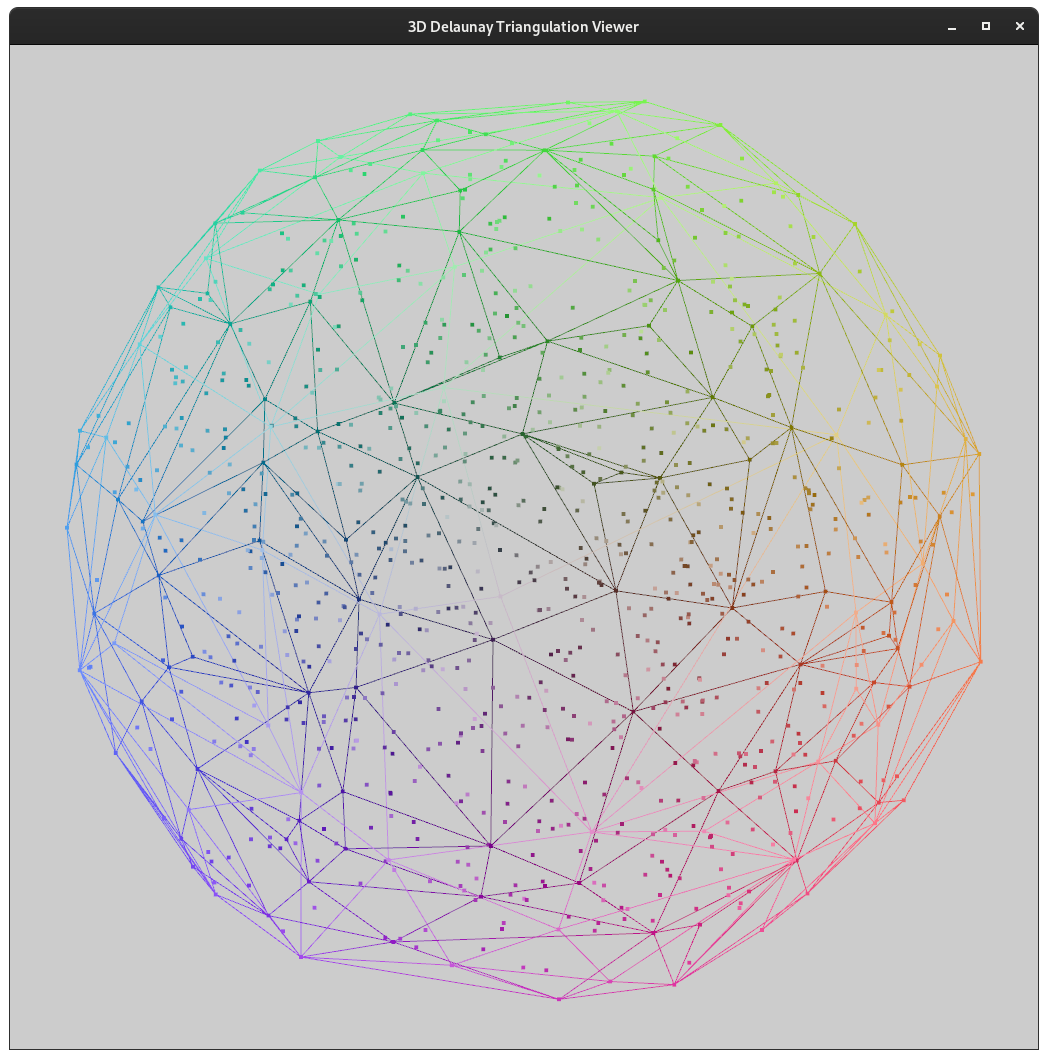
\includegraphics[width=0.8\textwidth]{../../images/delaunay_3d_surface.png}
      \end{subfigure}
      \caption[]{%
        The left image shows a three-dimensional Delaunay tessellation of uniformly distributed points in the unit ball.
        All points are connected by using tetrahedrons.
        Using only the surface triangles, one can generate a Delaunay triangulation of the curved surface as seen in the right picture.
      }
    \end{figure*}

    \begin{figure*}
      \center
      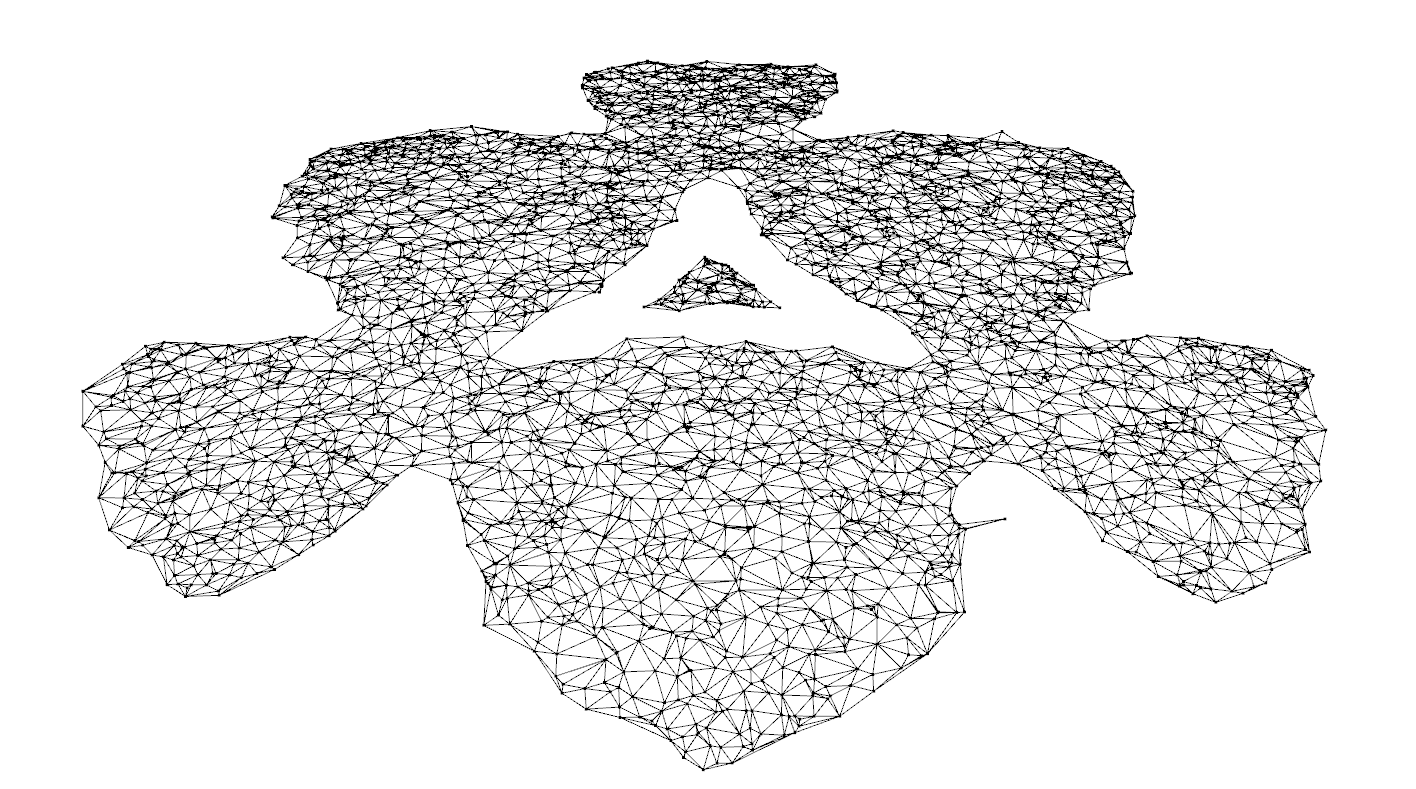
\includegraphics[width=0.7\textwidth]{../../images/3d_pareto_front_projected_tessellation.png}
      \caption[]{%
        The image shows a two-dimensional Delaunay triangulation of to-a-hyperplane projected curved Pareto surface in three-dimensional space from figure~\ref{fig:test-scene-2}.
        This procedure will be used to construct the surface of general curved Pareto frontiers.
      }
      \label{fig:delaunay-3d-projected}
    \end{figure*}
  % subsection delaunay_triangulation (end)
% section background (end)
\end{document}